\documentclass[10pt,a4paper]{article}
% for margining standards
\usepackage[left=3cm,right=3cm,top=3cm,bottom=3cm]{geometry}
% for counting references as a section
\usepackage[numbib,notlof,notlot,nottoc]{tocbibind}
% useful packages
\usepackage{
                graphicx, setspace, fontspec, caption,
                subcaption, float, polyglossia, rotating,
                lscape, pdflscape, indentfirst, tocloft,
                multirow, mathtools, currfile
            }
% paragraph related package
\usepackage[parfill]{parskip}
% use bzar font(THIS MUST BE LOADED BEFORE XePerian PACKAGE)
\setmainfont{BZar.ttf}
% the dear XePersian package
\usepackage{xepersian}
%
% General settings goes here.
%
% lines space
\renewcommand{\baselinestretch}{1.5}
% paragraph first line indention
\setlength{\parindent}{1cm}
% paragraph spacing
\setlength{\parskip}{1em}
% set graphics' path
\graphicspath{ {images/} }
% make table of content dotted
\renewcommand{\cftsecleader}{\cftdotfill{\cftdotsep}}
% define a new command as {half-space} in english
\newcommand{\halfspace}{\hspace{0pt}}
% define a new command as {half-space} in persian
\newcommand{\نیمفاصله}{\halfspace}
% define a shortcut for half-space in general
\renewcommand{\ }{\halfspace}
% define a new command for ease of use for rendering reference
\newcommand{\renderref}[1] { \begingroup \let\clearpage\relax \include{#1} \endgroup }
\newcommand{\مق}{\lr}
%
% DOCUMENT BEGIN
%
\begin{document}
\title{گزارش تمرین سوم
\\
طبقه\ بندی تصاویر با استفاده از\\
\lr{Convolutional Neural Network} و \lr{GoogleNet}
}
\author{داریوش حسن\ پور آده}
\date{۹۳۰۸۱۶۴}
\maketitle
\قسمت{قسمت ۱}
بنده ۶ عکس از محیط اطراف گرفتم را به شبکه دادم و نتایج\ اش به صورت زیر بدست آمد.\بند
\begin{figure}[h!]
\centering
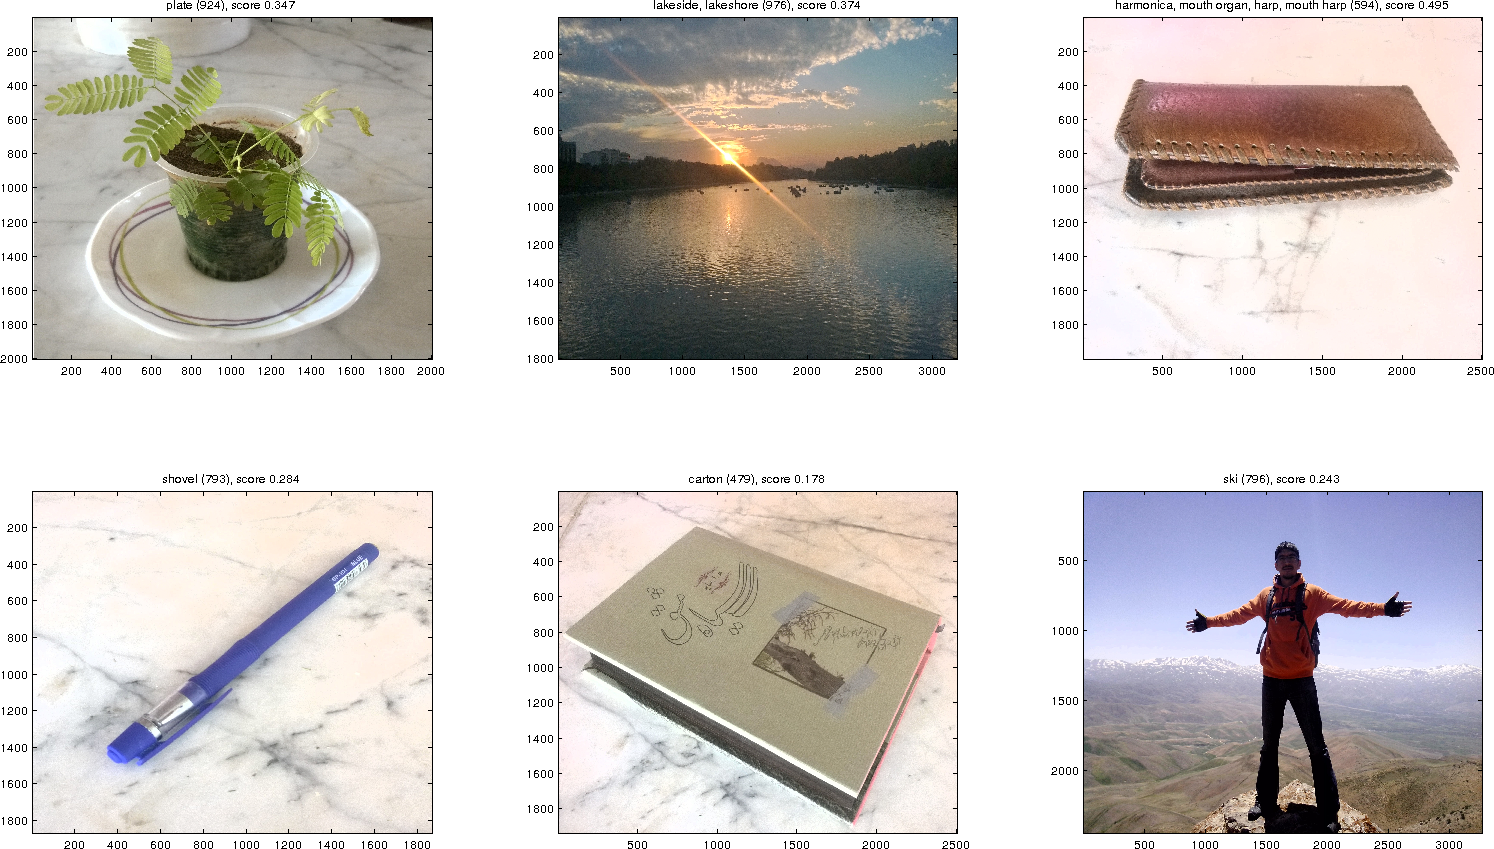
\includegraphics[width=\textwidth]{../sec_A/results/results}
\end{figure}
 که عکس اول(ردیف بالا، سمت راست) مربوط به «کیف پول» بنده می\ باشد که شبکه «سازدهنی» طبقه\ بندی است، عکس دوم مربوط که غروب خورشید که روی پل سی\ وسی پل گرفته شده است، که شبکه «دریاچه» طبقه\ بندی کرده است. عکس سوم مربوط به گیاهی است که در یک داخل یک زیراستکانی قرار داده شده است، که شبکه «بشقاب» طبقه\ بندی کرده است، عکس چهارم(ردیف پایین، سمت راست) مربوط به عکس بنده در ارتفاعات کوه\ ها می\ باشد، که شبکه «آسمان» طبقه\ بندی کرده است، عکس چهارم مربوط که به یک کتاب شعر از «هوشنگ ابتهاج» می\ باشد که شبکه «مقوا» طبقه\ بندی کرده است و آخر مربوط به یک عدد خودکار می\ باشد که شبکه «بیل» طبقه\ بندی کرده است.  همان\ طور که می\ بینیم به جز عکس آخر(خودکار) در مابقی عکس\ ها آنچه که شبکه طبقه\ بندی کرده است با آنچه که عکس\ ها بودند چندان هم بی\ ربط نیست، که نشان از خوب کار کردن شبکه\ ی \مق{GoogleNet} می\ باشد.
\قسمت{قسمت ۲}
در این قسمت عکس\ هایی که برای طبقه\ بندی در نظر گرفته است، عکس\ های \مق{MRI} مربوط به «مغز»\زیرنویس{۶۲ عدد عکس} و «زانو»\زیرنویس{۸۰ عدد عکس} می\ باشد که از موتور جستجوگر گوگل جمع\ آوری شده\ اند. همان\ طور که خواسته شده است ۸۰٪ از داده به صورت تصادفی به عنوان داده\ های آموزشی و ۲۰٪ مابقی را به عنوان داده\ های تست در نظر گرفته شدند. نتایج هر ۳ قسمت تکلیف در شکل زیر آمده است.
\begin{figure}[h!]
\centering
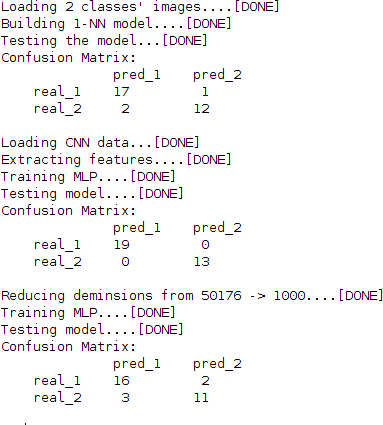
\includegraphics[scale=.8]{../sec_B/results/results}
\end{figure}
همان\ طور که در شکل بالا مشاهده می\ شود به ازای هر زیرقسمت(یعنی آموزش و ساخت مدل توسط «نزدیک\ ترین همسایه\زیرنویس{\مق{K-NN where K = 1}}»، استفاده از گوگل\ نت به عنوان استخراج کننده\ ی ویژگی و یک شبکه\ ی چندلایه و استفاده از \مق{‌PCA} و یک شبکه\ ی چندلایه) داده\ های تست را با استفاده از مدل بدست آمده تست کرده و \مق{Confusion Matrix} آن را رسم کرده\ ایم. برای اینکه بتوانیم نتایج حاصل از \مق{PCA} را با نتایج حاصل از گوگل\ نت مقایسه کنیم به تبعیت از ساختار شبکه\ ی گوگل\ نت عکس\ ها را از یک بردار ۵۰,۱۷۶ به یک بردار ۱۰۰۰ تایی کاهش دادیم و سپس توسط یک شبکه\ ی
$1000 \times 30 \times 1$
آموزش دادیم(همین ترکیب شبکه برای قسمت ۲.۲ تکلیف نیز در نظر گرفته شده است.). همان\ طور که می\ بینیم شبکه\ ای که با توسط گوگل\ نت کاهش بعد داده شده است بدون خطا همه\ ی داده\ های تست را به درستی طبقه\ بندی کرده است در حالی که هم در نزدیک\ ترین همسایه و هم در \مق{PCA} خطای طبقه\ بندی مشاهده می\ شود؛ که نشان می\ دهد گوگل\ نت می\ تواند کاهش\ بعد دهنده\ ی خوبی باشد.\بند
خروجی شبکه\ ی چندلایه در هردو قسمت ۲.۱ و ۲.۲ یک نورون بوده که برای کلاس یکی از دسته عکس\ ها مقدار هدف ۰ درنظر گرفته شده و برای دیگری ۱، در خروجی شبکه اگر بیشتر از ۰.۵ باشد ۱ در نظر گرفته می\ شود و اگر کمتر از ۰.۵ باشد ۰ در نظر گرفته می\ شود. در «نزدیک\ ترین همسایه» ۹٪ خطا، در «کاهش بعد با گوگل\ نت» ۰٪ خطا و در «کاهش بعد با \مق{PCA}» ۱۵٪ خطا داشته\ ایم، همان\ طور که می\ بینیم «کاهش\ بعد توسط گوگل\ نت و طبقه\ بندی توسط \مق{MLP}» حتی از «نزدیک\ ترین همسایه» نیز بهتر عمل کرده است.
\قسمت{قسمت ۳}
در این قسمت بنده عکس\ ها را دانلود کرده و برچسب\ های عکس\ های مرتبط با هر یک از عکس\ ها را استخراج کرده و سعی در ایجاد شبکه\ ای کانولشنی که بتواند بروی داده\ ها یادگیری انجام دهد کردم، کدهای مربوطه نوشته شده است(همراه مابقی تکلیف ارسال شده است) ولی نتوانستم ترکیبی صحیح برای شبکه بدست بیاورم و همش خطای
\vspace{-1.4em}\begin{center}\lr{Matrix dimensions must agree.}\end{center}\vspace{-1em}
میگیرم، هرکاری کردم نتوانستم ترکیب مناسبی بدون خطا بدست بیاورم -- حتی با نویسندگان این کتابخانه بابت راهنمایی تماس گرفتم، ولی باز هم در نتوانستم ترکیب صحیحی بدست بیاورم!!!
\end{document}
